\documentclass[handout]{beamer}
%Пакеты для математических символов:
\usepackage{amsmath} % американское математическое сообщество.
\usepackage{amssymb} % миллион разных значков и готический, ажурный шрифты.
\usepackage{amscd} % диаграммы, графики.
\usepackage{amsthm} % окружения теорем, определений и тд.
\usepackage{physics} % основные физические символы
%\usepackage{latexsym} % треугольники и пьяная стрелка.

%пакеты для шрифтов:
%\usepackage{euscript} % прописной шрифт с завитушками.
\usepackage{MnSymbol} % Значеки доказательства
\usepackage{verbatim} % улучшенный шрифт "пишущей машинки".
%\usepackage{array} % более удобные таблицы.
%\usepackage{multirow} % мультистолбцы в таблицах.
%\usepackage{longtable} % таблицы на несколько страниц.
%\usepackage{latexsym}

\usepackage{etoolbox}
\usepackage{slashbox} %Разделениени текста \backslashbox{}{}
\usepackage{collectbox} % Добавляет коробочки, можно складывать туда текст)

%Пакеты для оформления:
\RequirePackage[center, medium]{titlesec}% Стиль секций и заголовков
%\usepackage[x11names]{xcolor} % 317 новых цветов для текста.
%\usepackage{multicol} % набор текста в несколько колонн.
\usepackage{graphicx} % расширенные возможности вставки стандартных картинок.
\usepackage{subcaption} % возможность вставлять картинки в строчку
%\usepackage{caption} % возможность подавить нумерацию у caption.
\usepackage{wrapfig} % вставка картинок и таблиц, обтекаемых текстом.
\usepackage{cancel} % значки для сокращения дробей, упрощения, стремления.
%\usepackage{misccorr} % в заголовках появляется точка, но при ссылке на них ее нет.
%\usepackage{indentfirst} % отступ у первой строки раздела
%\usepackage{showkeys} % показывает label формул над их номером.
%\usepackage{fancyhdr} % удобное создание верхних и нижних колонтитулов.
%\usepackage{titlesec} % еще одно создание верхних и нижних колонтитулов

%Пакеты шрифтов, кодировок. НЕ МЕНЯТЬ РАСПОЛОЖЕНИЕ.
\usepackage[utf8]{inputenc} % кодировка символов.
%\usepackage{mathtext} % позволяет использовать русские буквы в формулах. НЕСОВМЕСТИМО С tempora.
\usepackage[T1, T2A]{fontenc} % кодировка шрифта.
\usepackage[english, russian]{babel} % доступные языки.



%Отступы и поля:
%размеры страницы А4 11.7x8.3in
\textwidth=7.3in % ширина текста
\textheight=10in % высота текста
\oddsidemargin=-0.5in % левый отступ(базовый 1дюйм + значение)
\topmargin=-0.5in % отступ сверху до колонтитула(базовый 1дюйм + значение)


%Сокращения
%Скобочки
\newcommand{\inrad}[1]{\left( #1 \right)}
\newcommand{\inner}[1]{\left( #1 \right)}
\newcommand{\infig}[1]{\left{ #1 \right}}
\newcommand{\insqr}[1]{\left[ #1 \right]}
\newcommand{\ave}[1]{\left\langle #1 \right\rangle}


%% Красивые <= и >=
\renewcommand{\geq}{\geqslant}
\renewcommand{\leq}{\leqslant}

%%Значек выполнятся
\newcommand{\per}{\hookrightarrow}


%% Более привычные греческие буквы
\renewcommand{\phi}{\varphi}
\renewcommand{\epsilon}{\varepsilon}
\newcommand{\eps}{\varepsilon}
\newcommand{\com}{\mathbb{C}}
\newcommand{\re}{\mathbb{R}}
\newcommand{\nat}{\mathbb{N}}
\newcommand{\stp}{$\filledmedtriangleleft$}
\newcommand{\enp}{$\filledmedsquare$}

\makeatletter
\newcommand{\sqbox}{%
    \collectbox{%
        \@tempdima=\dimexpr\width-\totalheight\relax
        \ifdim\@tempdima<\z@
            \fbox{\hbox{\hspace{-.5\@tempdima}\BOXCONTENT\hspace{-.5\@tempdima}}}%
        \else
            \ht\collectedbox=\dimexpr\ht\collectedbox+.5\@tempdima\relax
            \dp\collectedbox=\dimexpr\dp\collectedbox+.5\@tempdima\relax
            \fbox{\BOXCONTENT}%
        \fi
    }%
}
\makeatother
\newcommand{\mergelines}[2]{
\begin{tabular}{llp{.5\textwidth}}
#1 \\ #2
\end{tabular}
}
\newcommand\tab[1][0.51cm]{\hspace*{#1}}
\newcommand\difh[2]{\frac{\partial #1}{\partial #2}}


\usetheme{Madrid} % Выбор темы
\usecolortheme{seahorse} % Выбор цветовой схемы
\title{Эффект Керра}
\author{Карибджанов Матвей}

\begin{document}



\begin{frame}% первый слайд
    \titlepage
\end{frame}

\begin{frame}
    \frametitle{Проблема (эксперимент)}
    \begin{figure}[h]
        \centering
        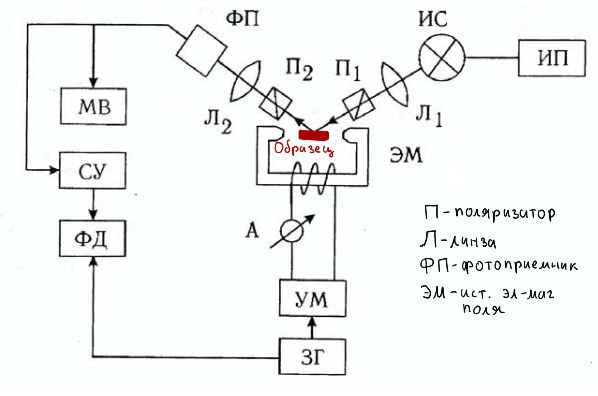
\includegraphics[width=1\textwidth]{exp.jpg}
    \end{figure}
\end{frame}


\begin{frame}
    \frametitle{Постановка задачи}
    \begin{columns}
        \begin{column}{0.5\textwidth}
            Пусть тезоры магнитной и электрической проницаемости:
            \begin{gather}
                \eps_{ij} = 
                \begin{pmatrix}
                    \eps& -i\eps M& 0\\
                    i\eps M& \eps& 0\\
                    0& 0& \eps_0
                \end{pmatrix}
            \end{gather}
            \begin{gather}
                \mu_{ij} = 
                \begin{pmatrix}
                    \mu& -i\mu M'& 0\\
                    i\mu M'& \mu& 0\\
                    0& 0& \mu_0
                \end{pmatrix}
            \end{gather}
        \end{column}

        \begin{column}{0.5\textwidth}
            \begin{eqnarray}
                \label{eq_max_1}
                e_{ijl} \partial_j H_l = \cfrac{1}{c} \partial_t D_i\\
                \label{eq_max_2}
                e_{ijl} \partial_j E_l = -\cfrac{1}{c} \partial_t B_i\\
                \label{eq_max_3}
                \partial_i D_i = 0\\
                \partial_i B_i = 0\\
                D_i = \eps_{ij} E_j\\
                B_i = \mu_{ij} H_j
            \end{eqnarray}
        \end{column}
      \end{columns}
\end{frame}


\begin{frame}
    \frametitle{Разновидности эффектов Керра}
    \begin{figure}[h]
        \centering
        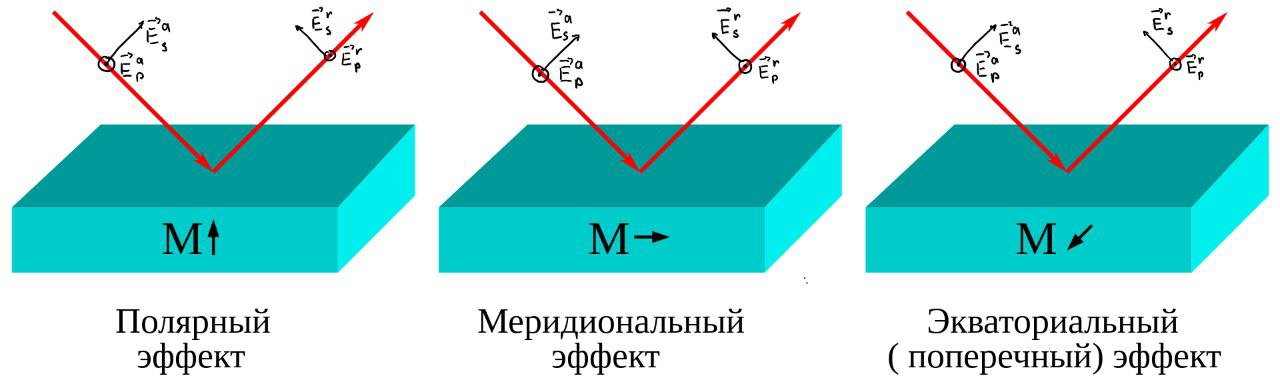
\includegraphics[width=1\textwidth]{kerr__.jpg}
    \end{figure}
\end{frame}


\begin{frame}
    \frametitle{Решение уравнений Максвелла}
    \begin{columns}
        \begin{column}{0.6\textwidth}
            Применив к \ref{eq_max_1} $e_{mqi} \partial_q$ получим:
            \begin{eqnarray*}
                e_{mqi} \partial_q e_{ijl} \partial_j H_l = 
                -\inner{\delta_{mj}\delta_{ql} - \delta_{ml}\delta_{qj}}
                \partial_q\partial_j H_l = \\
                = \partial_q\partial_q H_m - \partial_l\partial_m H_l = 
                (k_l k_m H_l - k_q k_q H_m)n^2 =\\
                = (k_m k_l H_l - H_m)n^2
            \end{eqnarray*}
            \begin{eqnarray*}
                \cfrac{1}{c}e_{mqi} \partial_q \partial_t \eps_{ij} E_j = 
                \cfrac{1}{c} i\omega e_{mqi} \partial_q \eps_{ij} E_j =\\
                = \cfrac{1}{c} \omega e_{mqi} k_q \eps_{ij} E_j
            \end{eqnarray*}
        \end{column}

        \begin{column}{0.35\textwidth}
            Из уравнения \ref{eq_max_2}:
            \begin{eqnarray*}
                e_{ijl} \partial_j E_l 
                = -i e_{ijl} k_j E_l
            \end{eqnarray*}
            \begin{eqnarray*}
                -\cfrac{1}{c}\partial_t B_i = 
                -\cfrac{1}{c}\partial_t \mu_{ij} H_j = \\
                = - \cfrac{i\omega}{c} \mu_{ij} H_j = 
                -\cfrac{i\omega}{c} B_i
            \end{eqnarray*}
            \begin{equation*}
                E_l = \cfrac{\omega}{c} (s^{-1})_{li}  B_i
            \end{equation*}
        \end{column}
      \end{columns}

      \begin{gather}
        s_{mi} = e_{mqi} k_q = 
        \begin{pmatrix}
            0& -k_z& k_y\\
            k_z& 0& -k_x\\
            -k_y& k_x& 0
        \end{pmatrix}
    \end{gather}
\end{frame}

\begin{frame}
    \frametitle{Ответ к уравнениям максвелла [2]}
    \begin{eqnarray}
        H_x + h_x h_i H^i = p\insqr{B_y\inner{m + \cfrac{\eps_0}{\eps} \inner{iMn_x - 1}} 
        + B_x\inner{\cfrac{h_x}{h_y}m + \cfrac{\eps_0}{\eps} \inner{n_x - iM}}}\\
        H_y + h_y h_i H^i = p\insqr{B_x\inner{m + \cfrac{\eps_0}{\eps} \inner{iMn_y - 1}} 
        + B_y\inner{\cfrac{h_y}{h_x}m + \cfrac{\eps_0}{\eps} \inner{n_y - iM}}}\\
        H_z - h_z h_i H^i = p\insqr{i\cfrac{\eps_0}{\eps} \inner{\cfrac{h_z}{h_y}B_y - \cfrac{h_z}{h_x}B_x}-
        \mu_0 M n_z H_z}M + \cfrac{\eps \mu_0}{n^2}H_z
    \end{eqnarray}
    Где введены следующие обозначения:
    \begin{eqnarray*}
        p = \cfrac{\eps^2 h_x h_y}{n^2 \inner{\eps_0 h_z^2 + \eps \inner{h_x^2 + h_z^2}}}, \
        h_i = \cfrac{c}{\omega} k_i, \ m = 1 - M^2, \ n_i = \cfrac{1 - h_i^2}{h_x h_y}, \\  
        B_x = \mu H_x - i\mu M' H_y, \ B_y = i\mu M' H_x + \mu H_y   
    \end{eqnarray*}
\end{frame}

\begin{frame}
    \frametitle{Первые результаты}
    Запросив требование к определителю $H = \hat A H \implies \det{A} = 0$:
    \begin{equation}
        n^2 = \eps_0 \mu_0 \inner{1 \mp h_z \inner{M - M'}}
    \end{equation}
    Пусть волна оладает $H_z \neq 0, \ H_x = H_y = 0$ что соответствует p поляризации: 
    \begin{equation}
        n_p^2  = \eps \mu_0 \inner{1 - M^2}  
    \end{equation}
    Для $H_z = 0, \ H_x \neq H_y \neq 0$:
    \begin{equation}
        n_s^2  = \eps_0 \mu \inner{1 - M'^2}  
    \end{equation}
\end{frame}

\begin{frame}
    \frametitle{Экваториальный эффект Керра}
    \begin{columns}
        \begin{column}{0.7\textwidth}
            Пусть падающая отраженная и прошедшая волны:
            \begin{gather*}
                H^a = \exp  \insqr{i\omega \inner{t - \cfrac{h_xx+h_yy}{c}n}}
                \begin{pmatrix}
                    -h_y A_s\\
                    h_x A_s\\
                    A_p
                \end{pmatrix}, \\
                H^r = \exp  \insqr{i\omega \inner{t - \cfrac{-h_xx+h_yy}{c}n}}       
                \begin{pmatrix}
                    -h_y R_s\\
                    -h_x R_s\\
                    R_p
                \end{pmatrix}, \\
                H^d = \exp  \insqr{i\omega \inner{t - \cfrac{h_xx+h_yy}{c}n}}      
                \begin{pmatrix}
                    D_1\\
                    D_2\\
                    D_3
                \end{pmatrix}
            \end{gather*}
        \end{column}

        \begin{column}{0.3\textwidth}
            \begin{figure}[h]
                \centering
                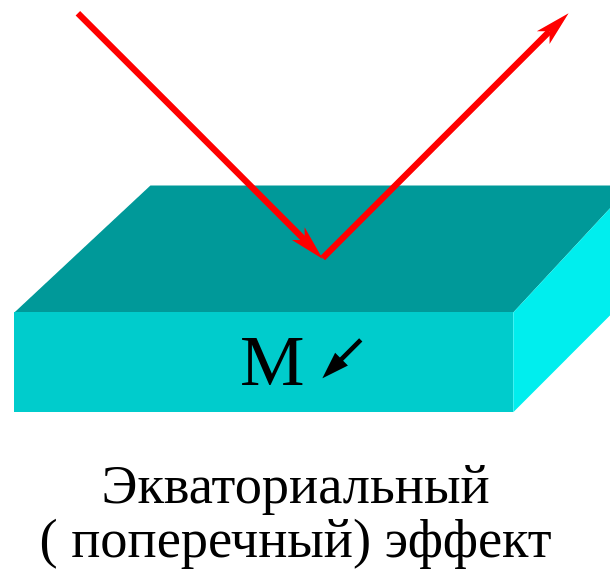
\includegraphics[width=1\textwidth]{ecvat_kerr.png}
            \end{figure}
        \end{column}
      \end{columns}
\end{frame}


\begin{frame}
    \frametitle{Поверхностные критерии}

        Для электрического поля получим:
        \begin{eqnarray*}
            E_y^a = \cfrac{h_x}{i\omega}A_p \exp{i\omega \tau_a}&
            E_z^a = -\cfrac{1}{i\omega} A_s \exp{i \omega \tau_a}\\
            E^r_y = -\cfrac{h_x}{i\omega} R_p \exp{i \omega \tau_r}&
            E_z^r = -\cfrac{1}{i\omega} R_s \exp{i \omega \tau_r}\\
        \end{eqnarray*}

        \begin{eqnarray*}
            E_y^d = \cfrac{n}{i\omega \eps} \cfrac{h_x + ih_y M}{1 - M^2}D_3 \exp{i \omega \tau_d}\\
            E_z^d = \cfrac{n}{i\omega \eps_0}\insqr{h_y D_1- h_x D_2}
        \end{eqnarray*}
\end{frame}

\begin{frame}
    \frametitle{Результаты}

        Учтя ганичныйе условия:
        \begin{eqnarray*}
            E_y^a + E_y^r = E^d_y& E_z^a + E_z^r = E^d_z \\
            H_y^a + H_y^r = H_y^d& H_z^a + H_z^r = H_z^d
        \end{eqnarray*}
        И найдя из \ref{eq_max_3} связь компонент векторав:
        \begin{equation*}
            D_1 = \cfrac{iM'h_x - h_b}{h_x + iM'h_y}D_2
        \end{equation*}
        Получим:
        \begin{eqnarray}
            \cfrac{R_s}{A_s} = \cfrac{h_x n_s - \eps_0 \inner{h_x + iM'h_y}}{h_x n_s + \eps_0 \inner{h_x + iM'h_y}}\\
            \cfrac{R_p}{A_p} = \cfrac{h_x n_p - \mu_0 \inner{h_x + iMh_y}}{h_x n_p + \mu_0 \inner{h_x + iMh_y}}
        \end{eqnarray}
\end{frame}

\begin{frame}
    \frametitle{Пример [1]}
    \begin{columns}
        \begin{column}{0.5\textwidth}
            \begin{figure}[h]
                \centering
                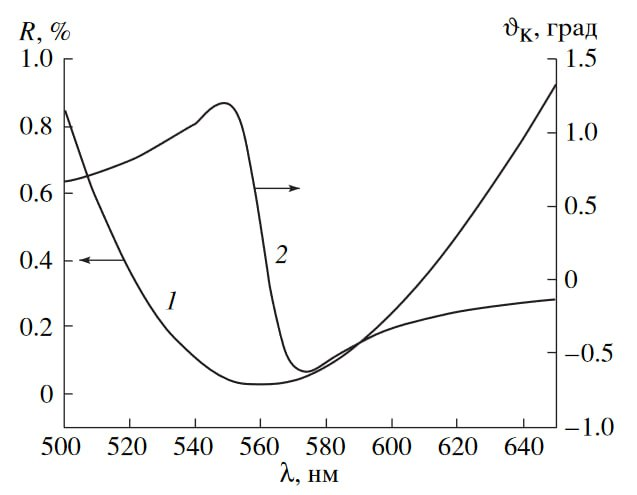
\includegraphics[width=1\textwidth]{init.jpg}
            \end{figure}
        \end{column}

        \begin{column}{0.5\textwidth}
            \begin{figure}[h]
                \centering
                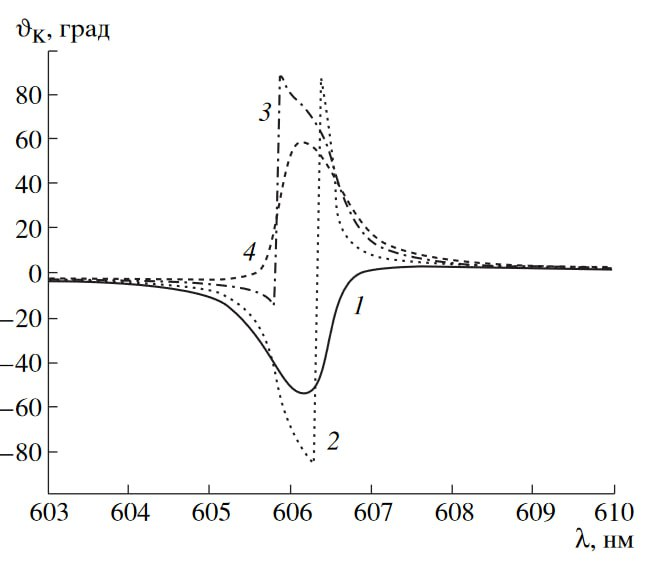
\includegraphics[width=1\textwidth]{mag_field.jpg}
            \end{figure}
        \end{column}
      \end{columns}
\end{frame}

\begin{frame}
    \frametitle{Пример \ref{exp}}
    \begin{figure}[h]
        \centering
        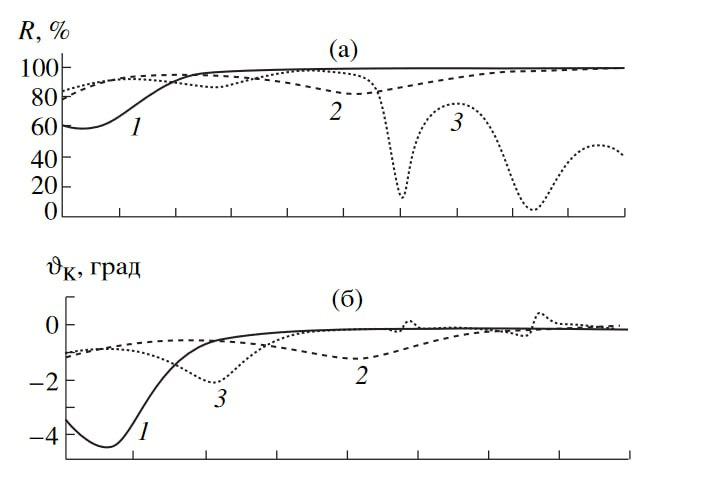
\includegraphics[width=1\textwidth]{samp.jpg}
    \end{figure}
\end{frame}

\begin{frame}
    \frametitle{Источники}
    \begin{itemize}
        \item[1] Vinogradov A.P., Erokhin S.G., Granovskiǐ A.B., Inoue M. Journal of Communications Technology and Electronics. 2004. Т. 49. № 6. С. 682-685. \label{exp}
        \item[2] \label{theor} Кринчик Г.С. Физика магнитных явлений. — М.: из-во МГУ, 1985. — 336 с.
    \end{itemize}
    
\end{frame}

\end{document}